%% ═══════════════════════════════════════════════════════════════════════════
%% MODERN OPERATING SYSTEMS (MOS) — COMPREHENSIVE STUDY NOTES & THEORY GUIDE
%% APJ Abdul Kalam Technological University / CET S5
%% Styled with Anthropic Notes Design System
%% ═══════════════════════════════════════════════════════════════════════════

\documentclass[11pt,a4paper]{article}

%% ─── Packages ────────────────────────────────────────────────────────────────
\usepackage{fontspec}

%% Font configuration with local fonts and synthetic fallbacks
\setmainfont{Anthropic-serif}[
    Path          = ./,
    Extension     = .ttf,
    AutoFakeBold  = 1.5,
    AutoFakeSlant = 0.2
]
\setsansfont{Poppins}[
    AutoFakeBold  = 1.5,
    AutoFakeSlant = 0.2
]
\setmonofont{DejaVu Sans Mono}[Scale=MatchLowercase]

\usepackage[margin=2.0cm, top=2.5cm, bottom=2.5cm, headheight=25pt]{geometry}
\usepackage[table]{xcolor}
\usepackage{tikz}
\usetikzlibrary{shapes.geometric, arrows.meta, positioning, fit, backgrounds,
                decorations.pathreplacing, decorations.pathmorphing, calc, patterns, shadows}
\usepackage{listings}
\usepackage{tcolorbox}
\tcbuselibrary{listings, skins, breakable, raster}
\usepackage{fancyhdr}
\usepackage{titlesec}
\usepackage{titletoc}
\usepackage{enumitem}
\usepackage{booktabs}
\usepackage{tabularx}
\usepackage{array}
\usepackage{microtype}
\usepackage{hyperref}
\usepackage{amssymb}
\usepackage{amsmath}
\usepackage{parskip}
\usepackage{colortbl}

%% ─── Document Metadata ──────────────────────────────────────────────────────
\newcommand{\docsubject}{CST305: Operating Systems (S5 CSE/CET)}
\newcommand{\docshortsubject}{MOS · S5 Notes}
\newcommand{\doctitle}{Operating Systems: Principles, Processes \& Concurrency}
\newcommand{\docauthor}{Sudheesh}

%% ─── Widow / Orphan Protection ──────────────────────────────────────────────
\widowpenalty=10000
\clubpenalty=10000

%% ─── Spacing ────────────────────────────────────────────────────────────────
\setlength{\parskip}{0.45em plus 0.15em minus 0.1em}
\setlength{\parindent}{0pt}

%% ─── Table Geometry ─────────────────────────────────────────────────────────
\setlength{\aboverulesep}{0pt}
\setlength{\belowrulesep}{0pt}
\setlength{\extrarowheight}{0.65ex}
\renewcommand{\arraystretch}{1.4}
\setlength{\arrayrulewidth}{0.4pt}

\newcolumntype{L}[1]{>{\raggedright\arraybackslash}p{#1}}
\newcolumntype{C}[1]{>{\centering\arraybackslash}p{#1}}
\newcolumntype{R}[1]{>{\raggedleft\arraybackslash}p{#1}}

%% ─── Brand Colors (Anthropic Palette) ────────────────────────────────────────
\definecolor{AnthDark}{HTML}{141413}
\definecolor{AnthLight}{HTML}{faf9f5}
\definecolor{AnthMidGray}{HTML}{7a7870}
\definecolor{AnthLightGray}{HTML}{e8e6dc}
\definecolor{AnthOrange}{HTML}{d97757}
\definecolor{AnthBlue}{HTML}{3b75a4}
\definecolor{AnthGreen}{HTML}{5d7343}
\definecolor{AnthCodeBG}{HTML}{edebe1}
\definecolor{AnthCardBG}{HTML}{f6f5ee}

\arrayrulecolor{AnthMidGray!40}

%% ─── Hyperref ────────────────────────────────────────────────────────────────
\hypersetup{
  colorlinks  = true,
  linkcolor   = AnthBlue,
  urlcolor    = AnthOrange,
  citecolor   = AnthGreen,
  pdftitle    = {\doctitle{} · \docsubject},
  pdfauthor   = {\docauthor},
}

%% ─── Page Style ─────────────────────────────────────────────────────────────
\pagestyle{fancy}
\fancyhf{}
\fancyhead[L]{\small\sffamily\color{AnthMidGray}\textbf{\doctitle} \textbar\ \docshortsubject}
\fancyhead[R]{\small\sffamily\color{AnthMidGray}\thepage}
\renewcommand{\headrulewidth}{0.4pt}
\renewcommand{\headrule}{%
  \hbox to\headwidth{\color{AnthOrange}\leaders\hrule height \headrulewidth\hfill}}
\renewcommand{\footrulewidth}{0.4pt}
\renewcommand{\footrule}{%
  \hbox to\headwidth{\color{AnthLightGray}\leaders\hrule height \footrulewidth\hfill}}
\fancyfoot[L]{\footnotesize\sffamily\color{AnthMidGray} APJ Abdul Kalam Technological University (KTU S5)}
\fancyfoot[R]{\footnotesize\sffamily\color{AnthMidGray} MOS Comprehensive Study Material}

%% ─── Section Formatting ─────────────────────────────────────────────────────
\titleformat{\section}
  {\Large\bfseries\sffamily\color{AnthDark}}
  {\colorbox{AnthOrange}{\makebox[0.65cm][c]{\color{white}\thesection}}\quad}
  {0em}
  {}
  [\vspace{-0.5ex}\color{AnthLightGray}\hrule\vspace{0.4ex}]

\titleformat{\subsection}
  {\large\bfseries\sffamily\color{AnthDark}}
  {\color{AnthBlue}\thesubsection\enspace}
  {0em}{}

\titleformat{\subsubsection}
  {\normalsize\bfseries\sffamily\color{AnthDark}}
  {\color{AnthGreen}\thesubsubsection\enspace}
  {0em}{}

\titlespacing{\section}     {0pt}{1.5em}{0.6em}
\titlespacing{\subsection}  {0pt}{1.1em}{0.3em}
\titlespacing{\subsubsection}{0pt}{0.8em}{0.25em}

%% ─── Table of Contents Styling ──────────────────────────────────────────────
\contentsmargin{0pt}

\titlecontents{section}
  [0pt]
  {\vspace{4pt}\bfseries\sffamily\color{AnthDark}}
  {\colorbox{AnthOrange}{\makebox[0.55cm][c]{\color{white}\small\thecontentslabel}}\enspace}
  {}
  {\hfill\color{AnthOrange}\contentspage}

\titlecontents{subsection}
  [1.5em]
  {\small\sffamily\color{AnthBlue}}
  {\thecontentslabel\enspace}
  {}
  {\titlerule*[6pt]{\tiny\color{AnthMidGray}.}\color{AnthBlue}\contentspage}

\titlecontents{subsubsection}
  [3.5em]
  {\footnotesize\sffamily\color{AnthGreen}}
  {\thecontentslabel\enspace}
  {}
  {\titlerule*[6pt]{\tiny\color{AnthMidGray}.}\color{AnthGreen}\contentspage}

%% ─── Code Listings ───────────────────────────────────────────────────────────
\lstset{
  language        = C,
  basicstyle      = \ttfamily\small,
  keywordstyle    = \color{AnthOrange}\bfseries,
  stringstyle     = \color{AnthGreen},
  commentstyle    = \color{AnthMidGray}\itshape,
  numberstyle     = \tiny\color{AnthMidGray},
  numbers         = left,
  stepnumber      = 1,
  numbersep       = 10pt,
  breaklines      = true,
  tabsize         = 4,
  showstringspaces= false,
  frame           = none,
  xleftmargin     = 18pt,
  xrightmargin    = 6pt,
  aboveskip       = 4pt,
  belowskip       = 4pt,
  keepspaces      = true,
}

%% ─── tcolorbox Styles ────────────────────────────────────────────────────────
\tcbset{
  codebox/.style={
    enhanced, breakable,
    colback     = AnthDark,
    colframe    = AnthDark,
    arc         = 5pt,
    outer arc   = 5pt,
    left        = 6pt, right = 6pt, top = 6pt, bottom = 6pt,
    boxrule     = 0.6pt,
    colupper    = AnthLight,
    coltitle    = white,
    colbacktitle= AnthDark!90,
    fonttitle   = \small\bfseries\sffamily,
    attach boxed title to top left={yshift=-2mm, xshift=8mm},
    boxed title style={arc=3pt, colback=AnthDark!90, boxrule=0pt},
    drop fuzzy shadow=AnthMidGray!30,
    top         = 8pt,
  },
  notebox/.style={
    enhanced, breakable,
    colback     = AnthCardBG,
    colframe    = AnthMidGray!50,
    arc         = 5pt,
    left        = 10pt, right = 10pt, top = 8pt, bottom = 8pt,
    boxrule     = 0.6pt,
    colupper    = AnthDark,
    fonttitle   = \bfseries\sffamily,
    coltitle    = AnthDark,
    colbacktitle= AnthLightGray,
    borderline west={3.5pt}{0pt}{AnthMidGray},
    drop fuzzy shadow=AnthMidGray!20,
  },
  tipbox/.style={
    enhanced, breakable,
    colback     = AnthGreen!6,
    colframe    = AnthGreen!60,
    arc         = 5pt,
    left        = 10pt, right = 10pt, top = 8pt, bottom = 8pt,
    boxrule     = 0.6pt,
    colupper    = AnthDark,
    fonttitle   = \bfseries\sffamily,
    coltitle    = white,
    colbacktitle= AnthGreen,
    borderline west={3.5pt}{0pt}{AnthGreen},
    drop fuzzy shadow=AnthGreen!15,
  },
  warnbox/.style={
    enhanced, breakable,
    colback     = AnthOrange!6,
    colframe    = AnthOrange!60,
    arc         = 5pt,
    left        = 10pt, right = 10pt, top = 8pt, bottom = 8pt,
    boxrule     = 0.6pt,
    colupper    = AnthDark,
    fonttitle   = \bfseries\sffamily,
    coltitle    = white,
    colbacktitle= AnthOrange,
    borderline west={3.5pt}{0pt}{AnthOrange},
    drop fuzzy shadow=AnthOrange!15,
  },
  defbox/.style={
    enhanced, breakable,
    colback     = AnthLight,
    colframe    = AnthLightGray,
    arc         = 5pt,
    left        = 10pt, right = 10pt, top = 8pt, bottom = 8pt,
    boxrule     = 0.6pt,
    colupper    = AnthDark,
    borderline west={3.5pt}{0pt}{AnthOrange},
    drop fuzzy shadow=AnthMidGray!20,
  },
}

%% ─── Inline Helpers ──────────────────────────────────────────────────────────
\newcommand{\ic}[1]{\mbox{\colorbox{AnthCodeBG}{\footnotesize\ttfamily\textcolor{AnthBlue}{#1}}}}

\newcommand{\concept}[1]{%
  \noindent\textcolor{AnthGreen}{\rule{3pt}{10pt}}\enspace
  \textbf{\color{AnthDark}#1}\par\vspace{2pt}%
}

%% ─── List Style ──────────────────────────────────────────────────────────────
\setlist[itemize,1]{itemsep=2pt, topsep=3pt, parsep=0pt, label={\color{AnthOrange}\small$\blacktriangleright$}}
\setlist[itemize,2]{itemsep=2pt, topsep=2pt, parsep=0pt, label={\color{AnthBlue}\small$\blacktriangleright$}}
\setlist[itemize,3]{itemsep=1pt, topsep=1pt, parsep=0pt, label={\color{AnthGreen}\small$\blacktriangleright$}}

\setlist[enumerate,1]{itemsep=2pt, topsep=3pt, parsep=0pt, label={\color{AnthOrange}\arabic*.}}
\setlist[enumerate,2]{itemsep=2pt, topsep=2pt, parsep=0pt, label={\color{AnthBlue}\alph*)}}
\setlist[enumerate,3]{itemsep=1pt, topsep=1pt, parsep=0pt, label={\color{AnthGreen}\roman*.}}

%% ─── Custom Environments ─────────────────────────────────────────────────────
\newenvironment{Note}[1][Note]{\begin{tcolorbox}[notebox, title={#1}]}{\end{tcolorbox}}
\newenvironment{Tip}[1][Key Takeaway]{\begin{tcolorbox}[tipbox, title={#1}]}{\end{tcolorbox}}
\newenvironment{Warn}[1][Important Pitfall / Warning]{\begin{tcolorbox}[warnbox, title={#1}]}{\end{tcolorbox}}
\newenvironment{Def}[1][]{\begin{tcolorbox}[defbox]\ifx&#1&\else\textbf{#1:}\enspace\fi}{\end{tcolorbox}}

%% ─── Title Page ──────────────────────────────────────────────────────────────
\newcommand{\maketitlepage}{%
  \begin{titlepage}
    \pagecolor{AnthDark}
    \color{AnthLight}
    \vspace*{3.5cm}
    \begin{center}
      {\Huge\bfseries\sffamily \doctitle}\\[0.8em]
      {\Large\sffamily\color{AnthOrange} \docsubject}\\[2.5em]
      \color{AnthMidGray}\rule{0.45\textwidth}{0.4pt}\\[2.0em]
      {\large\sffamily Prepared for Semester 5 Examination}\\[0.5em]
      {\normalsize\sffamily\color{AnthLightGray} College of Engineering Trivandrum (CET)}\\[2.5em]
      {\small\sffamily\color{AnthMidGray} Author: \textbf{\docauthor} \quad\textbar\quad Compiled: \today}
    \end{center}
    \vfill
  \end{titlepage}
  \pagecolor{AnthLight}
  \color{AnthDark}
}

%% ═══════════════════════════════════════════════════════════════════════════
%% DOCUMENT BODY
%% ═══════════════════════════════════════════════════════════════════════════
\begin{document}

\maketitlepage

%% ─── Table of Contents ───────────────────────────────────────────────────────
\thispagestyle{empty}
{
  \hypersetup{hidelinks}
  \tableofcontents
}
\newpage

%% ─────────────────────────────────────────────────────────────────────────────
\section{Introduction to Operating Systems}
%% ─────────────────────────────────────────────────────────────────────────────

\subsection{Definition and Role of an Operating System}

\begin{Def}[Operating System (OS)]
An \textbf{Operating System} is system software that manages and handles both hardware and software resources of a computing device, acting as an intermediary and abstract interface between the user/applications and the underlying physical hardware.
\end{Def}

An Operating System operates as a \textbf{Resource Manager} and an \textbf{Extended Machine}:
\begin{itemize}
    \item \textbf{Resource Management:} Controls and allocates computing resources such as the Central Processing Unit (CPU), primary/secondary memory (RAM, disk), and file storage.
    \item \textbf{User-Hardware Interface:} Provides an abstraction layer hiding the raw, complex hardware details (registers, interrupt controllers, buses) and presenting a clean, convenient execution environment.
    \item \textbf{Core System Services:} Executes foundational management functions including process lifecycle handling, memory allocation, device communication, file systems, and system protection.
    \item \textbf{Organizational Analogy:} Organizes and coordinates diverse system resources much like government ministries or administrative departments manage state infrastructure.
    \item \textbf{Prominent Real-World Examples:} Linux, UNIX, Microsoft Windows 11, MS-DOS, Android, Apple macOS, iOS.
\end{itemize}

\subsection{Abstract System Architecture}

A computing system is conceptually organized into hierarchical layers. The OS resides between user application programs and physical hardware, ensuring isolated and governed execution.

\begin{center}
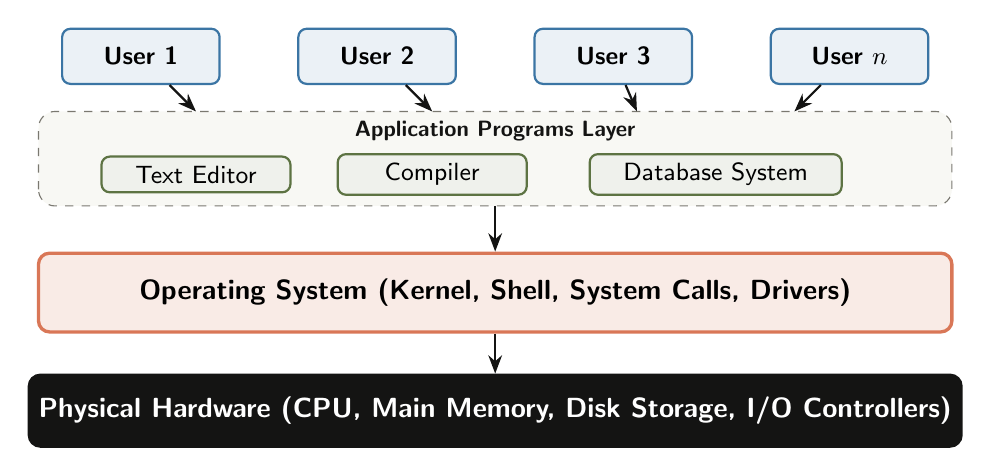
\begin{tikzpicture}[
    box/.style={draw=AnthDark, rounded corners=3pt, thick, align=center, fill=white, drop shadow={opacity=0.15}},
    userbox/.style={draw=AnthBlue, rounded corners=3pt, fill=AnthBlue!10, thick, align=center, font=\small\sffamily\bfseries},
    appbox/.style={draw=AnthGreen, rounded corners=3pt, fill=AnthGreen!10, thick, align=center, font=\small\sffamily},
    osbox/.style={draw=AnthOrange, rounded corners=4pt, fill=AnthOrange!15, very thick, align=center, font=\normalsize\sffamily\bfseries},
    hwbox/.style={draw=AnthDark, rounded corners=4pt, fill=AnthDark, very thick, align=center, font=\normalsize\sffamily\bfseries, text=white},
    arrow/.style={-{Stealth[scale=1.0]}, thick, color=AnthDark}
]

    %% Users
    \node[userbox, minimum width=2.0cm, minimum height=0.7cm] (u1) at (-4.5, 3.2) {User 1};
    \node[userbox, minimum width=2.0cm, minimum height=0.7cm] (u2) at (-1.5, 3.2) {User 2};
    \node[userbox, minimum width=2.0cm, minimum height=0.7cm] (u3) at (1.5, 3.2) {User 3};
    \node[userbox, minimum width=2.0cm, minimum height=0.7cm] (un) at (4.5, 3.2) {User $n$};

    %% Applications Container
    \draw[draw=AnthMidGray, dashed, fill=AnthLightGray!30, rounded corners=6pt] (-5.8, 1.3) rectangle (5.8, 2.5);
    \node[font=\footnotesize\sffamily\bfseries\color{AnthDark}] at (0, 2.25) {Application Programs Layer};

    \node[appbox, minimum width=2.4cm] (app1) at (-3.8, 1.7) {Text Editor};
    \node[appbox, minimum width=2.4cm] (app2) at (-0.8, 1.7) {Compiler};
    \node[appbox, minimum width=3.2cm] (app3) at (2.8, 1.7) {Database System};

    %% OS Layer
    \node[osbox, minimum width=11.6cm, minimum height=1.0cm] (os) at (0, 0.2) {Operating System (Kernel, Shell, System Calls, Drivers)};

    %% Hardware Layer
    \node[hwbox, minimum width=11.6cm, minimum height=0.9cm] (hw) at (0, -1.3) {Physical Hardware (CPU, Main Memory, Disk Storage, I/O Controllers)};

    %% Arrows
    \draw[arrow] (u1) -- (-3.8, 2.5);
    \draw[arrow] (u2) -- (-0.8, 2.5);
    \draw[arrow] (u3) -- (1.8, 2.5);
    \draw[arrow] (un) -- (3.8, 2.5);
    \draw[arrow] (0, 1.3) -- (os);
    \draw[arrow] (os) -- (hw);

\end{tikzpicture}
\end{center}

\subsection{Fundamental Components of an Operating System}

An Operating System is broadly structured into two primary operational entities:

\concept{1. The Shell (User Interface / Command Interpreter)}
\begin{itemize}
    \item The \textbf{outermost layer} of the operating system responsible for handling direct user interaction.
    \item Interprets user commands entered via a Command Line Interface (CLI) such as \ic{bash}, \ic{zsh}, or graphical gestures in a Graphical User Interface (GUI).
    \item Translates user commands into underlying system calls dispatched to the kernel, and formats output returned by the kernel for display.
\end{itemize}

\concept{2. The Kernel (Core Engine)}
\begin{itemize}
    \item The \textbf{central core component} that resides in main memory continuously from boot time.
    \item Operates in privileged mode (kernel/supervisor mode) with unrestricted hardware access.
    \item Acts as the primary interface between application software and low-level hardware devices, managing CPU scheduling, page tables, hardware interrupts, and device drivers.
\end{itemize}

%% ─────────────────────────────────────────────────────────────────────────────
\section{Core Functions of an Operating System}
%% ─────────────────────────────────────────────────────────────────────────────

The operating system coordinates multi-program execution, conceals complex hardware specifics through abstraction, enforces multi-tenant security, and maximizes hardware utilization.

\begin{center}
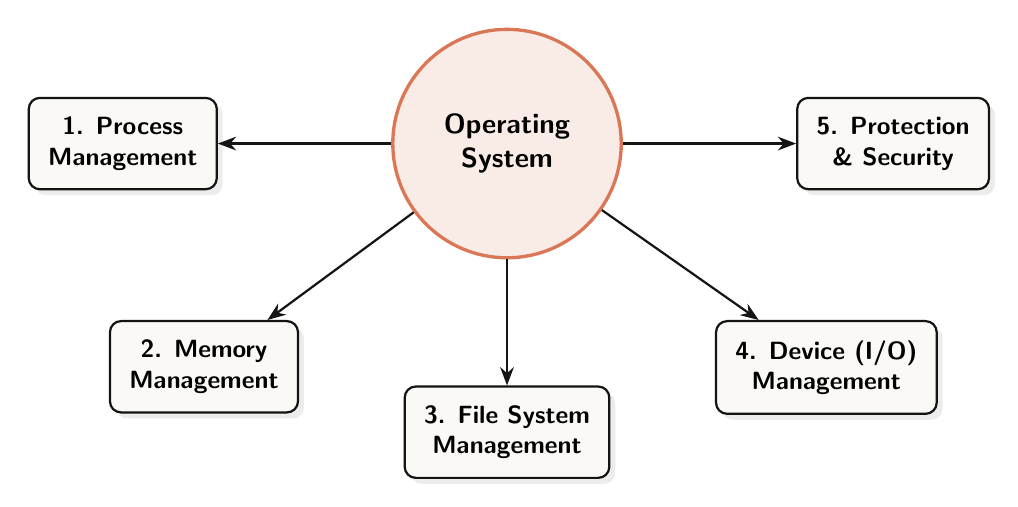
\begin{tikzpicture}[
    node distance=1.4cm and 1.8cm,
    core/.style={circle, draw=AnthOrange, fill=AnthOrange!15, very thick, align=center, font=\bfseries\sffamily, inner sep=12pt},
    fn/.style={rectangle, draw=AnthDark, fill=AnthLight, rounded corners=4pt, thick, align=center, font=\small\sffamily\bfseries, inner sep=7pt, drop shadow={opacity=0.15}},
    link/.style={-{Stealth[scale=1.0]}, thick, color=AnthDark}
]
    \node[core] (os) {Operating\\System};

    \node[fn, left=2.2cm of os] (proc) {1. Process\\Management};
    \node[fn, below left=1.2cm and 1.6cm of os] (mem) {2. Memory\\Management};
    \node[fn, below=1.6cm of os] (file) {3. File System\\Management};
    \node[fn, below right=1.2cm and 1.6cm of os] (dev) {4. Device (I/O)\\Management};
    \node[fn, right=2.2cm of os] (sec) {5. Protection\\\& Security};

    \draw[link] (os) -- (proc);
    \draw[link] (os) -- (mem);
    \draw[link] (os) -- (file);
    \draw[link] (os) -- (dev);
    \draw[link] (os) -- (sec);
\end{tikzpicture}
\end{center}

\subsection{1. Process Management}

A \textbf{process} is a program in active execution. Process management oversees process execution, concurrency, resource contention, and lifecycle transitions.

\begin{itemize}
    \item \textbf{CPU Scheduling:} Dynamically decides which ready process is allocated the CPU, choosing algorithms based on throughput, response time, and fairness.
    \item \textbf{Process Synchronization:} Controls concurrent access to shared mutable data using locks, semaphores, and monitors to prevent race conditions and non-deterministic execution.
    \item \textbf{Deadlock Handling:} Employs prevention, avoidance (Banker's algorithm), detection, and recovery schemes to resolve resource lockups where processes wait indefinitely for each other.
    \item \textbf{Inter-Process Communication (IPC):} Provides structured protocols (shared memory or message queues) allowing cooperative processes to exchange signals and data.
\end{itemize}

\subsection{2. Memory Management}

Memory management regulates how data is organized across the physical memory hierarchy (high-speed registers, cache, main memory/RAM, and secondary magnetic/solid-state storage).

\begin{center}
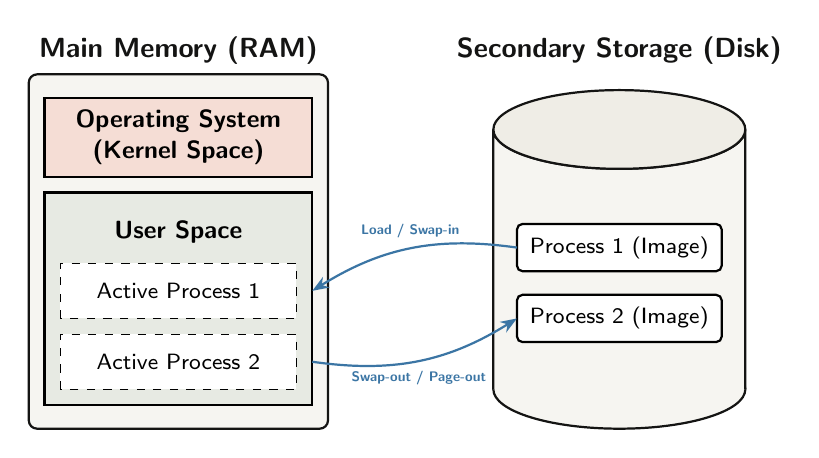
\begin{tikzpicture}[
    memblock/.style={draw=AnthDark, thick, align=center, font=\small\sffamily},
    arrow/.style={-{Stealth[scale=0.9]}, thick, color=AnthBlue}
]
    %% Main Memory RAM
    \draw[thick, draw=AnthDark, fill=AnthLightGray!40, rounded corners=3pt] (0,0) rectangle (3.8, 4.5);
    \node[font=\bfseries\sffamily\color{AnthDark}] at (1.9, 4.8) {Main Memory (RAM)};

    \draw[thick, fill=AnthOrange!25] (0.2, 3.2) rectangle (3.6, 4.2);
    \node[font=\small\sffamily\bfseries, align=center] at (1.9, 3.7) {Operating System\\(Kernel Space)};

    \draw[thick, fill=AnthGreen!15] (0.2, 0.3) rectangle (3.6, 3.0);
    \node[font=\small\sffamily\bfseries] at (1.9, 2.5) {User Space};
    \draw[dashed, fill=white] (0.4, 0.5) rectangle (3.4, 1.2);
    \node[font=\footnotesize\sffamily] at (1.9, 0.85) {Active Process 2};
    \draw[dashed, fill=white] (0.4, 1.4) rectangle (3.4, 2.1);
    \node[font=\footnotesize\sffamily] at (1.9, 1.75) {Active Process 1};

    %% Secondary Storage Disk
    \draw[thick, draw=AnthDark, fill=AnthLightGray!40] (7.5, 0.5) ellipse (1.6cm and 0.5cm);
    \draw[thick, draw=AnthDark, fill=AnthLightGray!40] (5.9, 0.5) -- (5.9, 3.8) arc (180:360:1.6cm and 0.5cm) -- (9.1, 0.5);
    \draw[thick, draw=AnthDark, fill=AnthLightGray!70] (7.5, 3.8) ellipse (1.6cm and 0.5cm);
    \node[font=\bfseries\sffamily\color{AnthDark}] at (7.5, 4.8) {Secondary Storage (Disk)};

    \draw[thick, fill=white, rounded corners=2pt] (6.2, 2.0) rectangle (8.8, 2.6);
    \node[font=\footnotesize\sffamily] at (7.5, 2.3) {Process 1 (Image)};

    \draw[thick, fill=white, rounded corners=2pt] (6.2, 1.1) rectangle (8.8, 1.7);
    \node[font=\footnotesize\sffamily] at (7.5, 1.4) {Process 2 (Image)};

    %% Swap Arrows
    \draw[arrow] (6.2, 2.3) to[bend right=20] node[above, font=\tiny\sffamily\bfseries, color=AnthBlue]{Load / Swap-in} (3.6, 1.75);
    \draw[arrow] (3.6, 0.85) to[bend right=20] node[below, font=\tiny\sffamily\bfseries, color=AnthBlue]{Swap-out / Page-out} (6.2, 1.4);

\end{tikzpicture}
\end{center}

\concept{Key Memory Management Activities}
\begin{enumerate}
    \item \textbf{Dynamic Allocation \& Deallocation:} Allocates memory blocks dynamically upon request (\ic{malloc()}, \ic{mmap()}) and reclaims space when released (\ic{free()}).
    \item \textbf{Memory Protection:} Enforces boundary checking via base and limit registers to prevent unauthorized processes from reading or overwriting other processes or kernel addresses.
    \item \textbf{Virtual Memory:} Maps contiguous virtual address spaces onto non-contiguous physical pages, utilizing backing disk swap space to execute programs larger than physical RAM.
    \item \textbf{Fragmentation Handling:} Minimizes internal and external fragmentation via dynamic relocation, paging, segmentation, and compaction.
    \item \textbf{Secondary Storage \& Disk Scheduling:} Organizes file blocks, tracks free-space bit vectors, and optimizes seek times using algorithms (FCFS, SSTF, SCAN/C-SCAN).
\end{enumerate}

\subsection{3. File System Management}

\begin{Def}[File System]
A collection of access methods, directory structures, and storage management mechanisms allowing uniform, persistent, named access to non-volatile secondary media.
\end{Def}

\begin{itemize}
    \item \textbf{File Attributes:} Name, identifier, type, physical location, size, protection permissions (read / write / execute), and timestamps (creation, last access, modification).
    \item \textbf{File Types:} Regular files (ASCII text, binary objects, executables), directory files, character/block device files, named pipes (FIFOs), and symbolic links.
    \item \textbf{Primitive Operations:} Create, Open, Read, Write, Seek (reposition), Truncate, Delete, and Close.
    \item \textbf{File Access Methods:}
    \begin{itemize}
        \item \emph{Sequential Access:} Information processed in order, byte by byte (e.g., tape drives, standard stream pipes).
        \item \emph{Direct (Random) Access:} Blocks read/written in arbitrary order by fixed logical record numbers (e.g., database tables).
        \item \emph{Indexed Access:} Uses an auxiliary index structure (e.g., B-Tree) for rapid keyed searches.
    \end{itemize}
\end{itemize}

\subsection{4. Device Management (I/O System)}

The I/O subsystem isolates hardware-specific quirks from the rest of the kernel, presenting a uniform device-driver interface.

\begin{center}
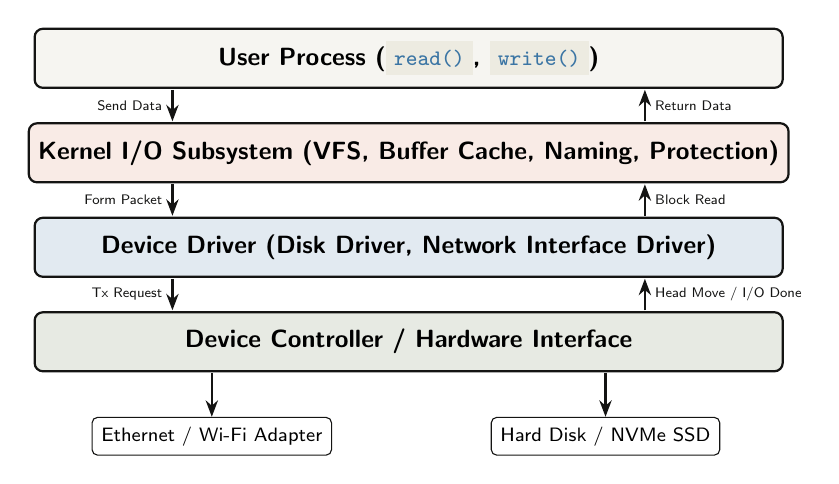
\begin{tikzpicture}[
    layer/.style={draw=AnthDark, fill=white, rounded corners=3pt, thick, align=center, minimum width=9.5cm, minimum height=0.75cm, font=\small\sffamily},
    arrow/.style={-{Stealth[scale=0.9]}, thick, color=AnthDark}
]
    \node[layer, fill=AnthLightGray!40, font=\small\sffamily\bfseries] (user) at (0, 3.6) {User Process (\ic{read()}, \ic{write()})};
    \node[layer, fill=AnthOrange!15, font=\small\sffamily\bfseries] (kernel) at (0, 2.4) {Kernel I/O Subsystem (VFS, Buffer Cache, Naming, Protection)};
    \node[layer, fill=AnthBlue!15, font=\small\sffamily\bfseries] (driver) at (0, 1.2) {Device Driver (Disk Driver, Network Interface Driver)};
    \node[layer, fill=AnthGreen!15, font=\small\sffamily\bfseries] (dev) at (0, 0.0) {Device Controller / Hardware Interface};

    %% Down/Up Arrows
    \draw[arrow] (-3.0, 3.2) -- (-3.0, 2.8) node[midway, left, font=\tiny\sffamily]{Send Data};
    \draw[arrow] (-3.0, 2.0) -- (-3.0, 1.6) node[midway, left, font=\tiny\sffamily]{Form Packet};
    \draw[arrow] (-3.0, 0.8) -- (-3.0, 0.4) node[midway, left, font=\tiny\sffamily]{Tx Request};

    \draw[arrow] (3.0, 2.8) -- (3.0, 3.2) node[midway, right, font=\tiny\sffamily]{Return Data};
    \draw[arrow] (3.0, 1.6) -- (3.0, 2.0) node[midway, right, font=\tiny\sffamily]{Block Read};
    \draw[arrow] (3.0, 0.4) -- (3.0, 0.8) node[midway, right, font=\tiny\sffamily]{Head Move / I/O Done};

    %% End devices
    \node[draw=AnthDark, fill=white, rounded corners=2pt, font=\scriptsize\sffamily] (eth) at (-2.5, -1.2) {Ethernet / Wi-Fi Adapter};
    \node[draw=AnthDark, fill=white, rounded corners=2pt, font=\scriptsize\sffamily] (disk) at (2.5, -1.2) {Hard Disk / NVMe SSD};

    \draw[arrow] (-2.5, -0.4) -- (eth);
    \draw[arrow] (2.5, -0.4) -- (disk);

\end{tikzpicture}
\end{center}

\concept{Major Mechanisms in I/O Management}
\begin{itemize}
    \item \textbf{Device Drivers:} Dedicated translation software routines that convert generic I/O requests (\ic{read\_block}) into hardware-specific controller register commands.
    \item \textbf{Buffering:} Temporary memory areas used to smooth speed mismatches between fast CPUs and slow peripheral devices, or reconcile differing data transfer sizes.
    \item \textbf{Caching:} Retains frequently referenced disk blocks in high-speed main memory to avoid repetitive physical I/O transfers.
    \item \textbf{Spooling (Simultaneous Peripheral Operations On-Line):} Intercepts data intended for dedicated, unshareable devices (e.g., printers). The OS buffers all print jobs onto disk, allowing the generating processes to finish immediately while the spooler daemon feeds the printer sequentially.
\end{itemize}

\subsection{5. Protection and Security}

\begin{Def}[Protection vs Security]
\textbf{Protection} refers to internal mechanisms controlling the access of programs, processes, or users to system resources. \textbf{Security} encompasses external and internal defenses safeguarding system integrity against unauthorized intrusion, data corruption, and malicious attacks.
\end{Def}

\begin{itemize}
    \item \textbf{Access Control:} Assigns privilege levels (Access Control Lists, POSIX \ic{rwx} bits) governing whether an entity may read, write, or execute a resource.
    \item \textbf{Authentication:} Positively validates user identity via identifiers (UID, SID), passwords, security tokens, or biometric parameters.
    \item \textbf{Resource Protection:} CPU dual-mode execution (User Mode vs Kernel Mode), memory protection keys, and I/O privilege isolation.
    \item \textbf{System Security:} Defends against malware, privilege escalation, Denial of Service (DoS/DDoS), and illicit data exfiltration.
\end{itemize}

%% ─────────────────────────────────────────────────────────────────────────────
\section{Process Concept, Lifecycle, and Management}
%% ─────────────────────────────────────────────────────────────────────────────

\subsection{Process Memory Address Space}

A process is more than passive program code (the text section). It represents an active execution instance containing program counters, registers, and specific memory segments.

\begin{center}
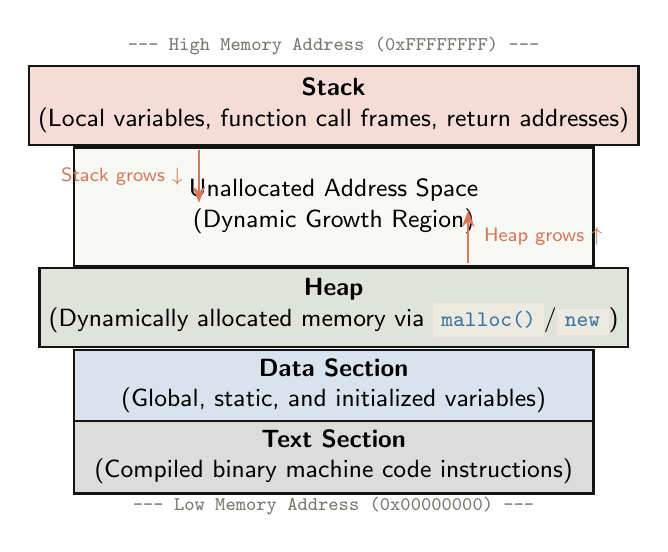
\begin{tikzpicture}[
    scale=0.95,
    seg/.style={draw=AnthDark, thick, minimum width=6.6cm, align=center, font=\small\sffamily},
    arrow/.style={-{Stealth[scale=0.9]}, thick, color=AnthOrange}
]
    %% Memory Boundary Indicator
    \node[font=\scriptsize\ttfamily\bfseries\color{AnthMidGray}] at (0, 4.8) {--- High Memory Address (0xFFFFFFFF) ---};
    
    %% Segments
    \node[seg, fill=AnthOrange!25, minimum height=1.0cm] (stack) at (0, 4.0) {\textbf{Stack}\\(Local variables, function call frames, return addresses)};
    \node[seg, fill=AnthLightGray!30, minimum height=1.5cm] (gap) at (0, 2.65) {Unallocated Address Space\\(Dynamic Growth Region)};
    \node[seg, fill=AnthGreen!20, minimum height=1.0cm] (heap) at (0, 1.3) {\textbf{Heap}\\(Dynamically allocated memory via \ic{malloc()}/\ic{new})};
    \node[seg, fill=AnthBlue!20, minimum height=0.9cm] (data) at (0, 0.25) {\textbf{Data Section}\\(Global, static, and initialized variables)};
    \node[seg, fill=AnthDark!15, minimum height=0.85cm] (text) at (0, -0.7) {\textbf{Text Section}\\(Compiled binary machine code instructions)};

    \node[font=\scriptsize\ttfamily\bfseries\color{AnthMidGray}] at (0, -1.35) {--- Low Memory Address (0x00000000) ---};

    %% Growth Arrows
    \draw[arrow] (-1.8, 3.4) -- (-1.8, 2.7) node[midway, left=2pt, font=\scriptsize\sffamily]{Stack grows $\downarrow$};
    \draw[arrow] (1.8, 1.9) -- (1.8, 2.6) node[midway, right=2pt, font=\scriptsize\sffamily]{Heap grows $\uparrow$};

\end{tikzpicture}
\end{center}

\subsection{Process States and 5-State Transition Model}

During its existence, a process moves through discrete execution states:
\begin{enumerate}
    \item \textbf{New:} The process is actively being created and initialized by the OS.
    \item \textbf{Ready:} The process is loaded in main memory, waiting to be allocated CPU time.
    \item \textbf{Running:} Instructions belonging to the process are being executed on the CPU.
    \item \textbf{Waiting (Blocked):} The process cannot execute until an external event occurs (e.g., I/O completion, timer signal, or lock acquisition).
    \item \textbf{Terminated:} The process has finished execution and its resources are released.
\end{enumerate}

\begin{center}
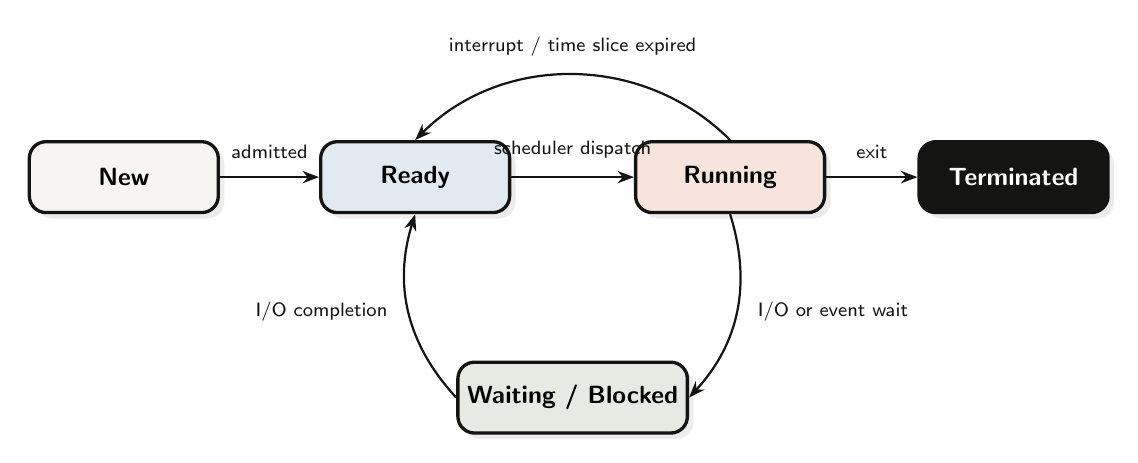
\begin{tikzpicture}[
    state/.style={draw=AnthDark, rounded corners=6pt, fill=AnthLight, very thick, minimum width=2.4cm, minimum height=0.9cm, font=\small\sffamily\bfseries, align=center, drop shadow={opacity=0.15}},
    arrow/.style={-{Stealth[scale=0.9]}, thick, color=AnthDark}
]
    \node[state, fill=AnthLightGray!40] (new) at (-5.5, 2.2) {New};
    \node[state, fill=AnthBlue!15] (ready) at (-1.8, 2.2) {Ready};
    \node[state, fill=AnthOrange!20] (running) at (2.2, 2.2) {Running};
    \node[state, fill=AnthDark, text=white] (term) at (5.8, 2.2) {Terminated};
    \node[state, fill=AnthGreen!15] (waiting) at (0.2, -0.6) {Waiting / Blocked};

    %% Transitions
    \draw[arrow] (new) -- (ready) node[midway, above=3pt, font=\scriptsize\sffamily]{admitted};
    \draw[arrow] (ready.east) -- (running.west) node[midway, above=3pt, font=\scriptsize\sffamily]{scheduler dispatch};
    \draw[arrow] (running.north) to[bend right=45] node[midway, above=3pt, font=\scriptsize\sffamily]{interrupt / time slice expired} (ready.north);
    \draw[arrow] (running) -- (term) node[midway, above=3pt, font=\scriptsize\sffamily]{exit};
    \draw[arrow] (running.south) to[bend left=30] node[midway, right=4pt, font=\scriptsize\sffamily]{I/O or event wait} (waiting.east);
    \draw[arrow] (waiting.west) to[bend left=30] node[midway, left=4pt, font=\scriptsize\sffamily]{I/O completion} (ready.south);

\end{tikzpicture}
\end{center}

\subsection{The Process Control Block (PCB)}

The \textbf{Process Control Block} (or Task Control Block) is the primary data structure maintained in kernel space for every active process.

\begin{center}
\begin{tabularx}{0.88\linewidth}{L{3.8cm} X}
  \rowcolor{AnthDark}
  \color{white}\textbf{PCB Field} & \color{white}\textbf{Description and Function} \\
  \rowcolor{AnthLightGray!60}
  \textbf{Pointer} & Linked list pointer linking the PCB into scheduling / device queues. \\
  \textbf{Process State} & Current lifecycle state (\ic{New}, \ic{Ready}, \ic{Running}, \ic{Waiting}, \ic{Terminated}). \\
  \rowcolor{AnthLightGray!60}
  \textbf{Process ID (PID)} & Unique positive integer identifying the process within the system. \\
  \textbf{Program Counter (PC)} & Address of the next binary instruction to be fetched and executed. \\
  \rowcolor{AnthLightGray!60}
  \textbf{CPU Registers} & Context save area for accumulators, index registers, stack pointers, and flags. \\
  \textbf{Memory Limits} & Base/limit register values, page tables, or segment descriptors. \\
  \rowcolor{AnthLightGray!60}
  \textbf{Scheduling Info} & Process priority, scheduling queue pointers, and aging counters. \\
  \textbf{Accounting Info} & CPU time consumed, wall-clock limits, account numbers, and thread counts. \\
  \rowcolor{AnthLightGray!60}
  \textbf{I/O Status Info} & List of allocated I/O devices, open file descriptors, and pending operations. \\
\end{tabularx}
\end{center}

\subsection{Operations on Processes: Creation and Termination}

\concept{1. Process Creation and UNIX Process Trees}
Operating systems create processes hierarchically. The initial creator is the \textbf{parent process}, and created instances are \textbf{child processes}, forming a directed tree rooted at \ic{systemd} or \ic{init} ($\text{PID}=1$).

\begin{center}
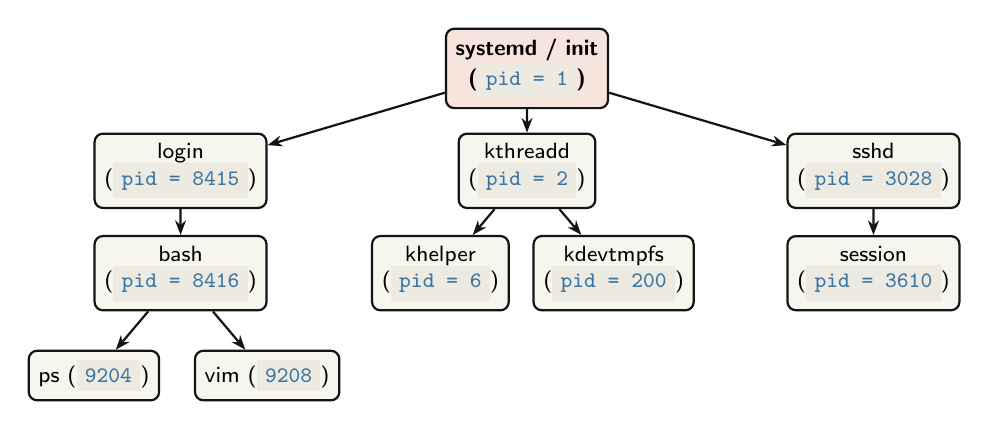
\begin{tikzpicture}[
    pnode/.style={draw=AnthDark, rounded corners=3pt, fill=AnthCardBG, thick, font=\footnotesize\sffamily, align=center, inner sep=3.5pt},
    edge from parent/.style={draw=AnthDark, thick, -{Stealth[scale=0.8]}},
    level 1/.style={sibling distance=4.4cm, level distance=1.3cm},
    level 2/.style={sibling distance=2.2cm, level distance=1.3cm}
]
    \node[pnode, fill=AnthOrange!20, font=\footnotesize\sffamily\bfseries] {systemd / init\\(\ic{pid = 1})}
        child {
            node[pnode] {login\\(\ic{pid = 8415})}
            child {
                node[pnode] {bash\\(\ic{pid = 8416})}
                child { node[pnode] {ps (\ic{9204})} }
                child { node[pnode] {vim (\ic{9208})} }
            }
        }
        child {
            node[pnode] {kthreadd\\(\ic{pid = 2})}
            child { node[pnode] {khelper\\(\ic{pid = 6})} }
            child { node[pnode] {kdevtmpfs\\(\ic{pid = 200})} }
        }
        child {
            node[pnode] {sshd\\(\ic{pid = 3028})}
            child { node[pnode] {session\\(\ic{pid = 3610})} }
        };
\end{tikzpicture}
\end{center}

\concept{Process Creation Options}
\begin{itemize}
    \item \textbf{Execution Alternatives:}
    \begin{enumerate}
        \item Parent executes concurrently with its child.
        \item Parent blocks and waits (\ic{wait()}) until some or all child processes terminate.
    \end{enumerate}
    \item \textbf{Address Space Alternatives:}
    \begin{enumerate}
        \item Child is an exact duplicate of the parent (inherits memory pages, open files via Copy-on-Write).
        \item Child has a new program loaded into its address space using \ic{exec()}.
    \end{enumerate}
    \item \textbf{Resource Partitioning:} Child obtains resources directly from the OS, or is restricted to a subset of parent resources to prevent runaway resource exhaustion.
\end{itemize}

\begin{tcolorbox}[codebox, title={UNIX Process Lifecycle using fork(), exec(), wait(), and exit()}]
\begin{lstlisting}[language=C]
#include <stdio.h>
#include <unistd.h>
#include <sys/types.h>
#include <sys/wait.h>

int main() {
    pid_t pid = fork(); // Fork returns 0 to child, child PID to parent

    if (pid < 0) {
        perror("Fork failed");
        return 1;
    } else if (pid == 0) {
        // Child Process
        printf("Child executing command...\n");
        execlp("/bin/ls", "ls", "-l", NULL); // Replaces address space
        _exit(0); // Called if exec fails
    } else {
        // Parent Process
        int status;
        wait(&status); // Blocks until child terminates
        printf("Parent resumed after child completion with status %d\n", status);
    }
    return 0;
}
\end{lstlisting}
\end{tcolorbox}

\concept{2. Process Termination and Cascading Termination}
\begin{itemize}
    \item A process concludes by executing \ic{exit(status)}, returning an integer exit status to its waiting parent.
    \item Operating systems reclaim all allocated physical/virtual memory, open file tables, and I/O buffers.
    \item \textbf{Cascading Termination:} In many OS environments, if a parent process terminates (normally or abnormally), all its child and descendant processes are forcefully terminated by the OS to prevent orphaned zombie trees.
\end{itemize}

%% ─────────────────────────────────────────────────────────────────────────────
\section{Process Schedulers}
%% ─────────────────────────────────────────────────────────────────────────────

A \textbf{Scheduler} is an OS component that selects processes from memory/disk queues and assigns CPU time to balance utilization, throughput, and response latency.

\begin{center}
\begin{tabularx}{\linewidth}{L{3.0cm} L{3.2cm} L{3.5cm} X}
  \rowcolor{AnthDark}
  \color{white}\textbf{Scheduler Type} &
  \color{white}\textbf{Alternative Name} &
  \color{white}\textbf{Frequency \& Speed} &
  \color{white}\textbf{Core Responsibility} \\
  \rowcolor{AnthLightGray!60}
  \textbf{Long-Term} & Job Scheduler & Infrequent (seconds/mins), Slow & Controls Degree of Multiprogramming; loads jobs from disk spool into RAM. \\
  \textbf{Short-Term} & CPU Scheduler & Frequent (10--100 ms), Extremely Fast & Selects next ready process in RAM and assigns CPU core. \\
  \rowcolor{AnthLightGray!60}
  \textbf{Medium-Term} & Swapper & Intermediate frequency & Swaps blocked/idle processes to disk to relieve RAM pressure; swaps in when ready. \\
\end{tabularx}
\end{center}

\begin{Tip}[Job Mix Balance]
The Long-Term Scheduler must maintain a balanced mix of \textbf{CPU-bound processes} (which spend most of their time computing) and \textbf{I/O-bound processes} (which spend most of their time waiting for I/O). If all jobs are I/O-bound, the ready queue is empty and the CPU sits idle; if all are CPU-bound, the I/O queue sits idle.
\end{Tip}

%% ─────────────────────────────────────────────────────────────────────────────
\section{Threads and Multithreading}
%% ─────────────────────────────────────────────────────────────────────────────

\subsection{Concept of Threads}

\begin{Def}[Thread]
A \textbf{Thread} (often called a \emph{Lightweight Process} or LWP) is the basic unit of CPU utilization. It comprises a unique Thread ID, a Program Counter (PC), a private Register Set, and an isolated Stack space, while sharing its Code section, Data section, and OS resources (e.g., open files) with peer threads of the same parent process.
\end{Def}

\begin{center}
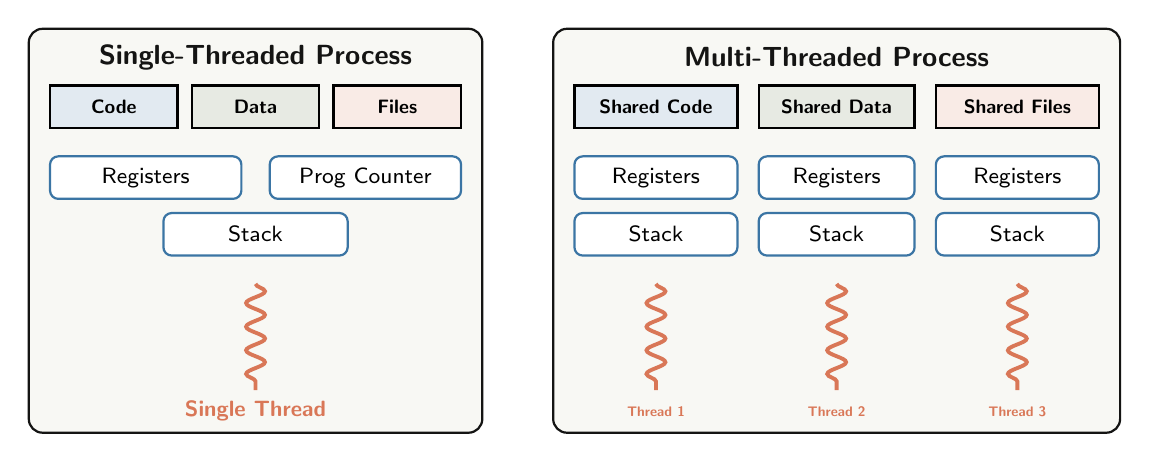
\begin{tikzpicture}[
    scale=0.9,
    box/.style={draw=AnthDark, thick, rounded corners=4pt, fill=AnthCardBG, align=center, font=\small\sffamily},
    tbox/.style={draw=AnthBlue, thick, rounded corners=3pt, fill=white, align=center, font=\footnotesize\sffamily},
    threadline/.style={draw=AnthOrange, line width=1.4pt, decorate, decoration={snake, amplitude=1.2mm, segment length=3mm}}
]
    %% Single Threaded Process
    \draw[thick, draw=AnthDark, fill=AnthLightGray!30, rounded corners=5pt] (-7.2, -2.5) rectangle (-0.8, 3.2);
    \node[font=\normalsize\sffamily\bfseries\color{AnthDark}] at (-4.0, 2.8) {Single-Threaded Process};

    \draw[thick, fill=AnthBlue!15] (-6.9, 1.8) rectangle (-5.1, 2.4) node[pos=.5, font=\scriptsize\sffamily\bfseries]{Code};
    \draw[thick, fill=AnthGreen!15] (-4.9, 1.8) rectangle (-3.1, 2.4) node[pos=.5, font=\scriptsize\sffamily\bfseries]{Data};
    \draw[thick, fill=AnthOrange!15] (-2.9, 1.8) rectangle (-1.1, 2.4) node[pos=.5, font=\scriptsize\sffamily\bfseries]{Files};

    \draw[tbox] (-6.9, 0.8) rectangle (-4.2, 1.4) node[pos=.5]{Registers};
    \draw[tbox] (-3.8, 0.8) rectangle (-1.1, 1.4) node[pos=.5]{Prog Counter};
    \draw[tbox] (-5.3, 0.0) rectangle (-2.7, 0.6) node[pos=.5]{Stack};

    \draw[threadline] (-4.0, -0.4) -- (-4.0, -1.9);
    \node[font=\footnotesize\sffamily\bfseries\color{AnthOrange}] at (-4.0, -2.2) {Single Thread};

    %% Multi Threaded Process
    \draw[thick, draw=AnthDark, fill=AnthLightGray!30, rounded corners=5pt] (0.2, -2.5) rectangle (8.2, 3.2);
    \node[font=\normalsize\sffamily\bfseries\color{AnthDark}] at (4.2, 2.8) {Multi-Threaded Process};

    \draw[thick, fill=AnthBlue!15] (0.5, 1.8) rectangle (2.8, 2.4) node[pos=.5, font=\scriptsize\sffamily\bfseries]{Shared Code};
    \draw[thick, fill=AnthGreen!15] (3.1, 1.8) rectangle (5.3, 2.4) node[pos=.5, font=\scriptsize\sffamily\bfseries]{Shared Data};
    \draw[thick, fill=AnthOrange!15] (5.6, 1.8) rectangle (7.9, 2.4) node[pos=.5, font=\scriptsize\sffamily\bfseries]{Shared Files};

    %% Thread 1
    \draw[tbox] (0.5, 0.8) rectangle (2.8, 1.4) node[pos=.5]{Registers};
    \draw[tbox] (0.5, 0.0) rectangle (2.8, 0.6) node[pos=.5]{Stack};
    \draw[threadline] (1.65, -0.4) -- (1.65, -1.9);
    \node[font=\tiny\sffamily\bfseries\color{AnthOrange}] at (1.65, -2.2) {Thread 1};

    %% Thread 2
    \draw[tbox] (3.1, 0.8) rectangle (5.3, 1.4) node[pos=.5]{Registers};
    \draw[tbox] (3.1, 0.0) rectangle (5.3, 0.6) node[pos=.5]{Stack};
    \draw[threadline] (4.2, -0.4) -- (4.2, -1.9);
    \node[font=\tiny\sffamily\bfseries\color{AnthOrange}] at (4.2, -2.2) {Thread 2};

    %% Thread 3
    \draw[tbox] (5.6, 0.8) rectangle (7.9, 1.4) node[pos=.5]{Registers};
    \draw[tbox] (5.6, 0.0) rectangle (7.9, 0.6) node[pos=.5]{Stack};
    \draw[threadline] (6.75, -0.4) -- (6.75, -1.9);
    \node[font=\tiny\sffamily\bfseries\color{AnthOrange}] at (6.75, -2.2) {Thread 3};

\end{tikzpicture}
\end{center}

\subsection{Benefits and Need for Threads}

\begin{enumerate}
    \item \textbf{Enhanced Responsiveness:} In interactive GUI applications, a background thread handles heavy file I/O or network fetching while the UI thread remains completely responsive to user clicks.
    \item \textbf{Resource Sharing:} Peer threads naturally share the process's address space and open file table without requiring IPC setups.
    \item \textbf{Economy and Low Overhead:} Creating a thread is roughly 30$\times$ cheaper than creating a separate process; context switching between threads avoids expensive TLB/page-table invalidations.
    \item \textbf{Scalability on Multicore Systems:} Threads run simultaneously on multiple hardware processor cores, achieving genuine hardware parallelism.
\end{enumerate}

\subsection{User-Level Threads (ULT) vs Kernel-Level Threads (KLT)}

\begin{center}
\begin{tabularx}{\linewidth}{L{3.2cm} X X}
  \rowcolor{AnthDark}
  \color{white}\textbf{Feature} &
  \color{white}\textbf{User-Level Threads (ULT)} &
  \color{white}\textbf{Kernel-Level Threads (KLT)} \\
  \rowcolor{AnthLightGray!60}
  \textbf{Management Layer} & Implemented entirely by user-space thread libraries (e.g., POSIX pthreads, green threads). & Managed directly by the OS Kernel via system calls. \\
  \textbf{Kernel Awareness} & Kernel is unaware of individual threads; sees only the parent process. & Kernel maintains thread tables, scheduling individual threads across cores. \\
  \rowcolor{AnthLightGray!60}
  \textbf{Switching Speed} & Extremely fast; no mode switch to kernel required. & Slower; requires user-to-kernel mode switch overhead. \\
  \textbf{Blocking Calls} & If one thread executes a blocking system call, the \textbf{entire process blocks}. & A blocking system call in one thread does \textbf{not} block peer threads. \\
  \rowcolor{AnthLightGray!60}
  \textbf{Multiprocessing} & Cannot exploit multi-core CPUs; all threads share the process's assigned core. & Kernel schedules different threads onto distinct physical CPU cores concurrently. \\
\end{tabularx}
\end{center}

%% ─────────────────────────────────────────────────────────────────────────────
\section{Process Synchronization \& The Critical Section Problem}
%% ─────────────────────────────────────────────────────────────────────────────

\subsection{Independent vs Cooperative Processes}

\begin{itemize}
    \item \textbf{Independent Process:} Cannot affect or be affected by the execution of other processes. It shares no state or mutable data.
    \item \textbf{Cooperative Process:} Shares data, memory, or files with other processes. Requires synchronization to avoid inconsistent data states.
\end{itemize}

\subsection{The Critical Section Problem}

\begin{Def}[Critical Section (CS)]
A segment of code in which a process accesses and manipulates shared resources (such as shared variables, files, or hardware devices). Concurrent execution by multiple processes inside their critical sections without coordination produces \textbf{race conditions}.
\end{Def}

\begin{tcolorbox}[codebox, title={General Structure of a Synchronized Process}]
\begin{lstlisting}[language=C]
do {
    /* ENTRY SECTION: Request permission, acquire locks */
    
    // CRITICAL SECTION: Access shared variables / hardware
    
    /* EXIT SECTION: Release locks, notify waiting processes */
    
    // REMAINDER SECTION: Non-critical, independent computations
} while (true);
\end{lstlisting}
\end{tcolorbox}

\subsection{Three Mandatory Criteria for a Valid CS Solution}

Any algorithmic or hardware solution to the Critical Section problem must satisfy three strict requirements:

\concept{1. Mutual Exclusion}
If process $P_i$ is executing in its critical section, then no other processes can be executing in their critical sections simultaneously.

\concept{2. Progress}
If no process is executing in its critical section and some processes wish to enter, only those processes that are \textbf{not} executing in their remainder section can participate in deciding which will enter next, and this selection cannot be postponed indefinitely.

\concept{3. Bounded Waiting}
There must exist a bound (limit) on the number of times that other processes are allowed to enter their critical sections after a process has made a formal request to enter its critical section and before that request is granted (prevents starvation).

%% ─────────────────────────────────────────────────────────────────────────────
\section{Software Solutions for Two Processes}
%% ─────────────────────────────────────────────────────────────────────────────

\subsection{Algorithm 1: Strict Alternation (Turn Variable)}

In Algorithm 1, processes share a single common integer variable \ic{turn}, initialized to \ic{0} or \ic{1}.

\begin{tcolorbox}[codebox, title={Algorithm 1: Structure of Process $P_i$ (where $j = 1 - i$)}]
\begin{lstlisting}[language=C]
int turn = 0; // Shared variable

// Process Pi
do {
    while (turn != i); // Busy waiting (Spinlock)
    
    /* Critical Section */
    
    turn = j;          // Pass turn to Pj
    
    /* Remainder Section */
} while (1);
\end{lstlisting}
\end{tcolorbox}

\concept{Analysis of Algorithm 1}
\begin{itemize}
    \item \textbf{Mutual Exclusion:} Satisfied. Since \ic{turn} can be either 0 or 1, only one process can enter its CS at any moment.
    \item \textbf{Progress:} \textbf{VIOLATED.} Execution is tied to strict alternation. If $P_0$ exits its CS and has no desire to re-enter (remains in remainder section), $P_1$ enters once, sets $\text{turn} = 0$, and when $P_1$ wishes to re-enter, it is blocked forever waiting for $P_0$ to change \ic{turn}.
\end{itemize}

\subsection{Algorithm 2: Flag Array (Signaling Intent)}

To eliminate strict alternation, Algorithm 1's single turn variable is replaced by a boolean array \ic{flag[2]}, initialized to \ic{false}.

\begin{tcolorbox}[codebox, title={Algorithm 2: Structure of Process $P_i$ (where $j = 1 - i$)}]
\begin{lstlisting}[language=C]
boolean flag[2] = {false, false}; // Shared array

// Process Pi
do {
    flag[i] = true;    // Signal intent to enter CS
    while (flag[j]);   // Wait if Pj is also ready or in CS
    
    /* Critical Section */
    
    flag[i] = false;   // Reset intent upon exit
    
    /* Remainder Section */
} while (1);
\end{lstlisting}
\end{tcolorbox}

\concept{Analysis of Algorithm 2}
\begin{itemize}
    \item \textbf{Mutual Exclusion:} Satisfied.
    \item \textbf{Progress:} \textbf{VIOLATED (Deadlock).} If $P_0$ and $P_1$ both set \ic{flag[0] = true} and \ic{flag[1] = true} concurrently before reaching the \ic{while} check, both evaluate the condition to \ic{true}, entering an infinite mutual spinlock where neither can progress.
\end{itemize}

\subsection{Algorithm 3: Peterson's Algorithm}

\begin{Def}[Peterson's Solution]
Peterson's Algorithm is a classic software-based solution for two processes that combines the key ideas of Algorithm 1 (turn variable) and Algorithm 2 (flag array).
\end{Def}

\begin{tcolorbox}[codebox, title={Peterson's Algorithm for Process $P_i$ and Process $P_j$}]
\begin{lstlisting}[language=C]
int turn;
boolean flag[2] = {false, false};

// Process Pi (i = 0, j = 1 or vice-versa)
do {
    flag[i] = true;                // State intent to enter
    turn = j;                      // Be courteous: offer turn to Pj
    while (flag[j] && turn == j);  // Busy wait while Pj wants CS and has turn
    
    /* CRITICAL SECTION */
    
    flag[i] = false;               // Reset flag on exit
    
    /* REMAINDER SECTION */
} while (true);
\end{lstlisting}
\end{tcolorbox}

\concept{Formal Correctness Proof}
\begin{enumerate}
    \item \textbf{Mutual Exclusion:} For both $P_0$ and $P_1$ to be in their CS simultaneously, both \ic{flag[0]} and \ic{flag[1]} must be \ic{true}, and both \ic{turn == 1} and \ic{turn == 0} must hold simultaneously, which is logically impossible.
    \item \textbf{Progress:} A process $P_i$ is prevented from entering only if \ic{flag[j] == true} and \ic{turn == j}. If $P_j$ does not want to enter, $\text{flag}[j] = \text{false}$, allowing $P_i$ to enter immediately.
    \item \textbf{Bounded Waiting:} If $P_j$ exits and wishes to re-enter, it must execute $\text{turn} = i$, immediately granting $P_i$ entry after at most one turn.
\end{enumerate}

\begin{Warn}[Modern Hardware Limitations of Peterson's Algorithm]
Peterson's Algorithm assumes sequential consistency. On modern superscalar multicore architectures, optimizing compilers and out-of-order execution hardware reorder independent memory reads and writes (\ic{flag[i]=true} and \ic{turn=j}). This breaks Peterson's algorithm unless explicit \textbf{Memory Barriers / Fences} (\ic{mfence}, atomic variables) are enforced.
\end{Warn}

%% ─────────────────────────────────────────────────────────────────────────────
\section{Inter-Process Communication (IPC)}
%% ─────────────────────────────────────────────────────────────────────────────

\subsection{Overview and Comparison of IPC Models}

Because processes execute in isolated virtual memory address spaces, the operating system provides two foundational IPC mechanisms:

\begin{center}
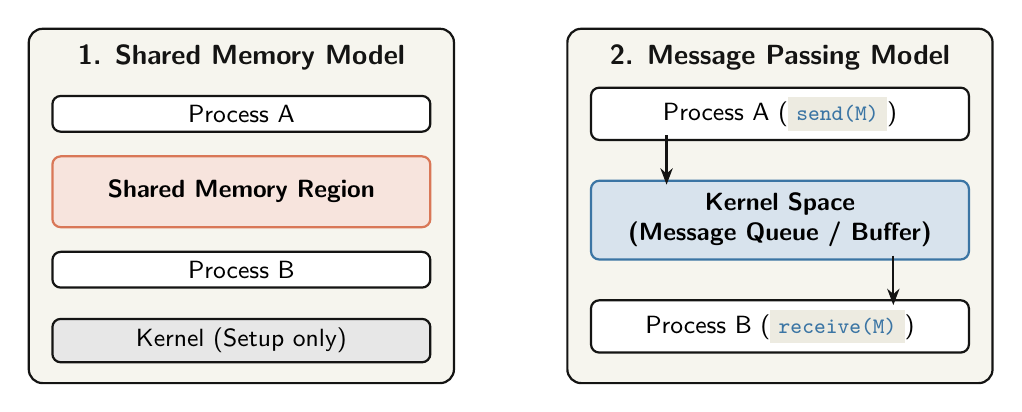
\begin{tikzpicture}[
    scale=0.9,
    box/.style={draw=AnthDark, thick, rounded corners=3pt, align=center, font=\small\sffamily},
    shbox/.style={draw=AnthOrange, fill=AnthOrange!20, thick, rounded corners=3pt, align=center, font=\small\sffamily\bfseries},
    msgbox/.style={draw=AnthBlue, fill=AnthBlue!20, thick, rounded corners=3pt, align=center, font=\small\sffamily\bfseries},
    arrow/.style={-{Stealth[scale=0.9]}, thick, color=AnthDark}
]
    %% Model 1: Shared Memory
    \draw[thick, draw=AnthDark, fill=AnthCardBG, rounded corners=5pt] (-6.8, -1.8) rectangle (-0.8, 3.2);
    \node[font=\normalsize\sffamily\bfseries\color{AnthDark}] at (-3.8, 2.8) {1. Shared Memory Model};

    \node[box, fill=white, minimum width=4.8cm] (pa1) at (-3.8, 2.0) {Process A};
    \node[shbox, minimum width=4.8cm, minimum height=0.9cm] (shmem) at (-3.8, 0.9) {Shared Memory Region};
    \node[box, fill=white, minimum width=4.8cm] (pb1) at (-3.8, -0.2) {Process B};
    \node[box, fill=AnthDark!10, minimum width=4.8cm] (k1) at (-3.8, -1.2) {Kernel (Setup only)};

    %% Model 2: Message Passing
    \draw[thick, draw=AnthDark, fill=AnthCardBG, rounded corners=5pt] (0.8, -1.8) rectangle (6.8, 3.2);
    \node[font=\normalsize\sffamily\bfseries\color{AnthDark}] at (3.8, 2.8) {2. Message Passing Model};

    \node[box, fill=white, minimum width=4.8cm] (pa2) at (3.8, 2.0) {Process A (\ic{send(M)})};
    \node[msgbox, minimum width=4.8cm, minimum height=1.0cm] (k2) at (3.8, 0.5) {Kernel Space\\(Message Queue / Buffer)};
    \node[box, fill=white, minimum width=4.8cm] (pb2) at (3.8, -1.0) {Process B (\ic{receive(M)})};

    \draw[arrow] (2.2, 1.7) -- (2.2, 1.0);
    \draw[arrow] (5.4, 0.0) -- (5.4, -0.7);

\end{tikzpicture}
\end{center}

\begin{center}
\begin{tabularx}{\linewidth}{L{3.2cm} X X}
  \rowcolor{AnthDark}
  \color{white}\textbf{Parameter} &
  \color{white}\textbf{Shared Memory Model} &
  \color{white}\textbf{Message Passing Model} \\
  \rowcolor{AnthLightGray!60}
  \textbf{Mechanism} & Address spaces overlap; processes read/write memory directly. & Information exchanged via kernel system calls (\ic{send()}, \ic{receive()}). \\
  \textbf{Kernel Involvement} & Only required during segment setup; zero kernel overhead during data transfer. & Kernel mediates every single message transfer. \\
  \rowcolor{AnthLightGray!60}
  \textbf{Speed \& Bandwidth} & Maximum memory-bus speed; ideal for massive data sets. & Moderate speed; context switches and buffer copies add latency. \\
  \textbf{Synchronization} & Must be explicitly handled by user application (semaphores, mutexes). & Built into system primitives (blocking/non-blocking). \\
  \rowcolor{AnthLightGray!60}
  \textbf{Distributed Setup} & Impractical across network boundaries (without distributed shared memory). & Easily implemented across network links and heterogeneous clusters. \\
\end{tabularx}
\end{center}

\subsection{Message Passing Operations and Communication Link Properties}

A message passing facility provides at least two basic primitive operations:
\begin{equation}
    \ic{send(message)} \quad \text{and} \quad \ic{receive(message)}
\end{equation}

\concept{1. Direct vs Indirect Communication}
\begin{itemize}
    \item \textbf{Direct Communication:} Senders and receivers explicitly name each other:
    \begin{itemize}
        \item \ic{send(P, message)} — Send a message directly to Process $P$.
        \item \ic{receive(Q, message)} — Receive a message from Process $Q$.
        \item Links are established automatically between pairs; symmetric addressing.
    \end{itemize}
    \item \textbf{Indirect Communication:} Messages are directed to and retrieved from shared mailboxes or ports (e.g., POSIX message queues with unique integer IDs):
    \begin{itemize}
        \item \ic{send(A, message)} — Send message to mailbox $A$.
        \item \ic{receive(A, message)} — Receive message from mailbox $A$.
    \end{itemize}
\end{itemize}

\concept{2. Synchronization Modes (Blocking vs Non-Blocking)}
\begin{itemize}
    \item \textbf{Blocking Send (Synchronous):} The sending process is suspended until the message is received by the destination process or mailbox.
    \item \textbf{Non-Blocking Send (Asynchronous):} The sending process deposits the message into the buffer and immediately resumes execution.
    \item \textbf{Blocking Receive (Synchronous):} The receiver blocks until a valid message arrives.
    \item \textbf{Non-Blocking Receive (Asynchronous):} The receiver retrieves either a valid waiting message or an immediate null status.
\end{itemize}

\subsection{Buffering Capacities in Message Passing}

Messages exchanged across communication links reside in temporary kernel queues implemented in one of three ways:

\begin{center}
\begin{tabularx}{\linewidth}{L{3.2cm} L{3.5cm} X}
  \rowcolor{AnthDark}
  \color{white}\textbf{Buffering Scheme} &
  \color{white}\textbf{Queue Capacity} &
  \color{white}\textbf{Operational Behavior} \\
  \rowcolor{AnthLightGray!60}
  \textbf{Zero Capacity} & Length = $0$ messages & Link cannot hold any waiting messages. Sender \textbf{must block} until receiver accepts the message (\textbf{Rendezvous}). \\
  \textbf{Bounded Capacity} & Finite length = $n$ messages & Holds up to $n$ messages. Sender continues immediately if space exists; sender blocks only if queue is full. \\
  \rowcolor{AnthLightGray!60}
  \textbf{Unbounded Capacity} & Infinite length ($\infty$) & Queue is dynamically sized. Sender \textbf{never blocks}; messages queue up indefinitely. \\
\end{tabularx}
\end{center}

%% ─────────────────────────────────────────────────────────────────────────────
\section{Summary Review \& Exam Booster Cheat Sheet}
%% ─────────────────────────────────────────────────────────────────────────────

\begin{Note}[Key Concepts Quick Summary]
\begin{itemize}
    \item \textbf{OS Definition:} Intermediary system software acting as a resource manager and abstract machine.
    \item \textbf{Two OS Components:} \textbf{Shell} (outer user interface / command interpreter) and \textbf{Kernel} (core engine managing CPU, memory, devices).
    \item \textbf{PCB Elements:} Pointer, Process State, PID, PC, CPU Registers, Memory Limits, Scheduling Info, Accounting, I/O Status.
    \item \textbf{Process States (5-State Model):} New $\to$ Ready $\rightleftharpoons$ Running $\to$ Terminated (with Waiting on I/O).
    \item \textbf{Process Lifecycle Calls:} \ic{fork()} clones process, \ic{exec()} loads program, \ic{wait()} blocks parent, \ic{exit()} terminates child.
    \item \textbf{Schedulers:} Long-Term (Degree of Multiprogramming), Short-Term (CPU assignment, high speed), Medium-Term (Swapper).
    \item \textbf{Threads (LWP):} Share code, data, open files; possess private stack, registers, and program counter.
    \item \textbf{Thread Types:} ULT (fast, user space, whole process blocks on I/O) vs KLT (kernel-managed, multicore capable, non-blocking).
    \item \textbf{Critical Section Criteria:} Mutual Exclusion, Progress, Bounded Waiting.
    \item \textbf{Peterson's Algorithm:} 2-process solution combining \ic{turn} and \ic{flag[2]}; satisfies all 3 criteria (requires memory barriers on modern CPUs).
    \item \textbf{IPC Models:} Shared Memory (fastest, user-synchronized) vs Message Passing (kernel-mediated, distributed-ready).
    \item \textbf{Message Buffering:} Zero (Rendezvous), Bounded (blocks when full), Unbounded (never blocks sender).
\end{itemize}
\end{Note}

\end{document}
